% v2-acmlarge-sample.tex, dated March 6 2012
% This is a sample file for ACM large trim journals
%
% Compilation using 'acmlarge.cls' - version 1.3, Aptara Inc.
% (c) 2011 Association for Computing Machinery (ACM)
%
% Questions/Suggestions/Feedback should be addressed to => "acmtexsupport@aptaracorp.com".
% Users can also go through the FAQs available on the journal's submission webpage.
%
% Steps to compile: latex, bibtex, latex latex
%
\documentclass[prodmode,acmtap]{acmlarge}

\usepackage[utf8x]{inputenc}
\usepackage[italian]{babel}
\usepackage{epstopdf}
\usepackage{graphicx}
\usepackage[hang,small,bf]{caption}
\usepackage{babel,blindtext}
%\usepackage{subcaption}



% Metadata Information
\acmVolume{1}
\acmNumber{1}
\acmArticle{1}
\articleSeq{1}
\acmYear{2013}
\acmMonth{6}

% Package to generate and customize Algorithm as per ACM style
\usepackage[ruled]{algorithm2e}
\SetAlFnt{\algofont}
\SetAlCapFnt{\algofont}
\SetAlCapNameFnt{\algofont}
\SetAlCapHSkip{0pt}
\IncMargin{-\parindent}
\renewcommand{\algorithmcfname}{ALGORITHM}


% Title portion
\title{Analisi della stabilità del protocollo di DHT Symphony\\
\Large{Relazione sul Progetto di Simulazione di Sistemi}
}
\author{MATTEO BRUCATO e MIRO MANNINO\affil{Università di Bologna}
}


\begin{abstract}
Symphony è un protocollo di overlay per sistemi peer-to-peer in grado di mantenere una tabella hash distribuita (DHT) attraverso nodi che risiedono in una rete geografica. In questa relazione daremo per prima cosa delle definizioni generali che aiutino l'analisi della stabilità in caso di churn, e forniscano uno strumento utile per la comparazione della stabilità di due protocolli differenti. Studieremo pertanto come il fenomeno di churn influenzi le latenze medie, i tempi dei messaggi e stabilità, in due modi differenti: variando la frequenza di join e variando il numero di peer che fanno join nello stesso istante. Mostreremo poi come tali misurazioni vengano influenzate utilizzando o meno il protocollo di re-linking. Infine calcoleremo il valore di $\epsilon^*$ di Symphony, in modo che questo possa essere utilizzato per comparare la sua stabilità con quella di altri protocolli di DHT.
\vspace*{50mm}
\end{abstract}

\category{}{}{}[]


\begin{document}


\maketitle


\section{Introduzione}
% Cos'è Sympony e cosa vogliamo verificare con la simulazione (stabilità, perché?)

Symphony~\cite{symphony} è un protocollo per tabelle hash distribuite (DHT) che, attraverso una rete di overlay costruita in base a particolari distribuzioni armoniche, è in grado di garantire lookup efficienti, poli-logaritmici nel numero di hop (salti), ovvero nella sua \emph{latenza}\footnote{In sintonia con la terminologia tipica della letteratura peer-to-peer, indichiamo col termine \emph{latenza} il numero medio di hop per l'operazione di lookup.}.

Attraverso un concetto denominato \emph{greedy routing} è stato mostrato come sia possibile indirizzare e consegnare un messaggio ad un qualsiasi nodo in una rete in al più $O(log^2 n)$ salti (un fenomeno chiamato anche \emph{Small World})~\cite{small-world}. Symphony si basa esattamente su questi concetti, i quali vengono applicati magistralmente al caso di reti peer-to-peer e al problema di creare DHT. In particolare, Symphony è in grado di garantire una latenza di $O(\frac{1}{k} log^2 n)$ salti, dove $k=O(1)$ è il numero di link che ogni nodo mantiene verso altri nodi della rete.

Nell'articolo in cui Symphony è stato presentato~\cite{symphony} vengono evidenziati i molteplici vantaggi del protocollo rispetto ai suoi predecessori (Chord, Viceroy, ecc.). Il vantaggio più evidente è quello di richiedere un numero costante $k=O(1)$ di link verso altri nodi della rete, a differenza di protocolli come Chord~\cite{chord} che richiedono un numero logaritmico di link uscenti.

Symphony, inoltre, è dimostrato essere \emph{scalabile} nella dimensione della rete, \emph{performante} rispetto alla latenza dei lookup, \emph{flessibile} rispetto ai sistemi in cui può essere integrato e \emph{semplice} per quanto riguarda l'implementazione.

Infine, gli autori dichiarano anche il sistema \emph{stabile}, ovvero capace di funzionare nel caso in cui gli host si uniscano alla rete ed escano dalla rete in maniera del tutto arbitraria, tipicamente con brevi periodi di vita. Ciononostante, un'approfondita analisi dell'articolo mostra come gli esperimenti effettuati per valutare la stabilità di Symphony offrano solamente una panoramica limitata sui possibili scenari che possano veramente essere fonte di instabilità. I test effettuati non sono tali da stressare il sistema fino ai punti più critici, in cui un'evidente instabilità possa essere misurata.

Lo scopo del presente elaborato è quello di studiare a fondo la stabilità del protocollo Symphony, e di stabilire in maniera più accurata se tale protocollo può essere veramente considerato stabile e in che misura. Più precisamente, ci poniamo l'obiettivo di valutare la stabilità del protocollo sotto carichi di stress causati da \emph{churn}, ovvero da alte frequenze di entrata e uscita dei nodi della rete. Studieremo sotto quali condizioni di stress la stabilità del protocollo vale e in quali condizioni essa comincia a vacillare.

Attraverso una serie di esperimenti in simulazione, e in particolare attraverso l'ausilio di un \emph{motore di churn} molto sofisticato, siamo in grado di stressare il sistema fino a mettere in luce alcuni evidenti sintomi di instabilità. I nostri esperimenti, infatti, mostrano che il protocollo Symphony è molto sensibile durante la fase di creazione della struttura di overlay atta a garantirne stabilità. Durante questa fase il numero di hop necessari ai lookup non è più garantito essere limitato superiormente dalla complessità asintotica dimostrata nel paper originale. Ciononostante, i sintomi di instabilità non sono preoccupanti, e il protocollo risponde comunque sufficientemente bene ad aumenti di traffico estremamente intensi. Il protocollo di re-linking permette inoltre al sistema di alleviare parecchio i sintomi di instabilità, poiché aiuta a mantenere la struttura in condizioni ottimali.

In questa relazione discutiamo anche alcuni principi generali per valutare la stabilità di protocolli DHT, e proponiamo alcune idee atte a valutare la stabilità di più protocolli DHT, i quali potrebbero essere utilizzati in futuro per esperimenti su più protocolli.

La relazione è organizzata nel seguente modo. In Sezione~\ref{symphony} descriveremo brevemente il protocollo Symphpny. In Sezione~\ref{stabilita} descriveremo formalmente il concetto di stabilità che sarà oggetto di valutazione del protocollo in esame. In Sezione~\ref{simulatore}, presenteremo i dettagli sul simulatore realizzato, il livello di astrazione del simulatore stesso e dettagli sulla sua realizzazione. La Sezione~\ref{risultati} raccoglierà i risultati sperimentali delle simulazioni, mentre la Sezione~\ref{conclusioni} illustrerà le nostre conclusioni.





\section{Il protocollo Symphony} \label{symphony}
% Breve introduzione ai termini del paper: join, leave, re-linking, ... tutto quello usato nel resto...
Symphony è un protocollo DHT basato su un'overlay strutturato con topologia ad anello. Gli identificatori dei nodi sono selezionati in maniera randomica uniforme nell'intervallo $[0,1)$. Ogni nodo $p_i$ con identificatore $x$ gestisce il sotto-intervallo dell'anello $(y,x]$, dove $y$ è l'identificatore del peer $p_{i-1}$ immediatamente precedente al peer $p_i$ (diremo che il peer $p_i$ gestisce un segmento di lunghezza $|x-y|$). In questo modo ogni valore $x \in [0,1)$ è gestito (univocamente) da uno ed un solo peer, che chiameremo il \emph{manager} di $x$ nel resto della presente relazione.

\subsection{Collegamenti tra nodi}
I nodi della rete Symphony sono collegati tra loro secondo due tipi di link: \emph{short link} e \emph{long link}, ovvero collegamenti a breve e lungo raggio. I collegamenti short servono a creare la struttura ad anello vera e propria: un peer $p_i$ è collegato per mezzo di due short link ai due peer $p_{i-1}$ e $p_{i+1}$ (supponendo sempre aritmetica modulo $n$), ovvero il suo predecessore e il suo successore nell'anello. I collegamenti long, invece, servono a permettere salti a lunga distanza nell'anello, i quali determinano la complessità poli-logaritmica del protocollo di routing di Symphony. I long link costituiscono quindi la caratteristica più importante del protocollo in esame.

Ogni nodo, dopo essere entrato nella rete di overlay creando i suoi 2 short link coi vicini, cerca di creare $k \ge 1$ long link uscenti. La decisione del peer con il quale collegarsi, per mezzo di un long link, viene fatta utilizzando un numero randomico $x \in [0,1)$, selezionato sulla base di una distribuzione di probabilità appartenente ad una famiglia di distribuzioni armoniche: una versione continua della distribuzione discreta di Kleinberg. A sua volta ogni peer può accettare al più $2k$ long link entranti, come stabilito dagli autori del protocollo. Pertanto, in reti molto affollate, può succedere che un peer cerchi per molte volte di creare long link con dei peer già saturi, fallendo costantemente. Gli autori impongono quindi un massimo numero di tentativi, lasciando la possibilità di avere meno di $k$ long link uscenti. I long link, sia entranti che uscenti, vengono visti in ogni modo bidirezionale: i link entranti vengono anche contati come uscenti.

\subsection{Join}
Quando un peer $p$ vuole entrare nella rete sceglie $x$, il proprio id, in maniera casuale, uniformemente nell'intervallo $[0,1)$. In seguito, $p$ cerca il peer $m(x)$, l'attuale manager di $x$, utilizzando una richiesta di lookup (il peer deve conoscere almeno un peer già presente nella rete per poterlo fare). Una volta trovato $m(x)$ il peer può entrare nella rete, distruggendo lo short link di $m(x)$ che lo collega al suo predecessore, e creandone altri due, ovvero inserendosi nel mezzo. Fatto ciò, il nuovo peer comincia la creazione dei suoi $k$ long link.


\subsection{Estimation Protocol}
La creazione dei long link prevede l'utilizzo di una funzione di distribuzione che prende in input $n$, il numero di peer attualmente nella rete. Symphony quindi prevede un protocollo per stimare il numero di peer presenti nella rete di overlay. Tale protocollo stima tale numero collezionando un insieme di $s$ lunghezze di segmenti e poi utilizzando la semplice formula $\frac{s}{X_s}$, dove $X_s$ denota la somma delle lunghezze dei segmenti. Gli autori stimano che $s = 3$ sia un numero sufficiente per avere una buona stima del numero dei peer presenti nella rete. Questi tre id vengono quindi recuperati in maniera del tutto gratuita dai peer coinvolti al momento del join. 

\subsection{Routing Protocol Bidirezionale}
Il Routing Protocol è il protocollo più importante di Symphony, poiché decide come instradare i messaggi di lookup all'interno della rete di overlay. Il protocollo prevede che i peer facciano il forward di un messaggio di lookup per l'id $x$ al vicino il cui id minimizza la distanza assoluta da $x$. Se invece il peer che riceve il messaggio di lookup gestisce già $x$, allora tale peer può già rispondere al mittente comunicandogli di essere il manager di $x$, mediante una comunicazione diretta. Esiste anche una versione del protocollo unidirezionale, meno performante, e che non prenderemo in esame nella presente relazione.

\subsection{Re-linking}
Il re-linking è un protocollo estremamente importante di Symphony, che permette di gestire al meglio le reti non statiche: i long link possono diventare obsoleti quando la rete subisce molti cambiamenti, ovvero quando cresce o diminuisce molto nel numero dei nodi. Si pensi ad esempio ai long link creati da un peer quanto la rete contava solamente pochi peer, e si pensi come questi siano inutili a fronte di una rete che è poi cresciuta del doppio. 

Il protocollo necessita che il peer $p_i$ mantenga due valori: $n_i$, la stima corrente del numero di peer, e $n^{link}_i$, la stima del numero dei peer al momento in cui i long link sono stati creati. Per evitare però che i long link vengano ricreati ogni volta che la rete subisce dei cambiamenti minimi nel numero (i.e. $n^{link}_i \neq n_i$), viene stabilito che vengano ricreati solamente quando $n_i / n^{link}_i \notin [1/2,2]$.

\section{Analisi della Stabilità} \label{stabilita}
% definizione formale e pochi esempi

Nell'articolo originale~\cite{symphony}, gli autori Manku et al. testano la stabilità del protocollo Symphony in una cosiddetta \emph{rete dinamica}, ovvero una rete in cui i nodi entrano ed escono arbitrariamente. In particolare, gli autori studiano una rete di centomila nodi, ognuno dei quali ha un numero logaritmico di vicini e alterna uno stato di attività ad uno stato di inattività. I tempi di attività e inattività sono tratti da due distribuzioni esponenziali diverse, tali che i nodi restino attivi per poco tempo (in media mezz'ora) e inattivi per il resto della giornata (23 ore e mezza in media). Le distribuzioni esponenziali fanno sì che la stragrande maggioranza dei nodi rispecchino questo comportamento.

Questo setup rispecchia certamente alcuni scenari veritieri di utilizzo dei sistemi DHT. I nodi entrano nella rete una volta al giorno e vi rimangono per pochissimo tempo (forse il tempo necessario per fare una semplice ricerca e scaricare uno o due file). Ciononostante non è certamente atto a coprire la maggioranza dei casi di utilizzo possibili, specialmente quelli in cui la rete venga stressata in maniera molto più pesante. Si pensi ad esempio ad un utilizzo di una DHT da parte di altri sistemi, in sistemi distribuiti integrati fra loro. In tali situazioni, non si può fare nessuna supposizione né sugli orari di utilizzo, né sulla durata d'utilizzo o sulla frequenza di entrata nella rete.

Non solo lo scenario usato nei test dagli autori di Symhony prevede una frequenza di entrata e uscita piuttosto basse, ma gli autori assumono anche una crescita della rete molto controllata. Nei loro test, infatti, essi fanno crescere la rete in maniera lineare durante l'arco di una giornata. Alla fine della prima giornata, tutti i centomila nodi sono entrati nella rete, e vi rimangono durante tutto l'arco della giornata successiva. Durante il terzo giorno, invece, i peer vengono fatti uscire dalla rete a intervalli regolari. Non siamo riusciti ad immaginare, in questo caso, un esempio di utilizzo reale che rispecchi questo particolare test. Ma soprattutto, ancora, questo test non è atto a stressare la rete con un'adeguata frequenza di churn, o in casi di altissima e imprevedibile attività.

Infine, i test riguardanti la stabilità presenti nell'articolo considerano solo reti senza re-linking. Reputiamo molto interessante stabilire cosa accade in una rete sotto churn nel caso in cui il re-linking sia attivo, in quanto esso forza molti peer a distruggere e ricreare tutti i propri long link, i quali sono quelli che contribuiscono maggiormente alle performance del protocollo stesso.


\subsection{Modello di stabilità}

Il modello di stabilità che vogliamo considerare nel presente elaborato è più complesso e a grana più fine di quello utilizzato nel paper originale. Innanzitutto, osserviamo come il tempo di permanenza di un certo peer nella rete è ininfluente rispetto la misura di stabilità della rete. Sapere che un peer sta nella rete per mezz'ora o per un giorno non fa alcuna differenza. Ciò che può maggiormente influire sulla stabilità è il fatto che una grande quantità di peer chiedano un lookup mentre la rete è in fase di creazione a seguito di \emph{join} (entrate) e \emph{leave} (uscite) dei peer.

L'ipotesi alla base dei nostri test è che durante i join (e/o i leave) l'anello di Symphony possa avere potenziali punti di inefficienza dati dal fatto che i peer che stanno entrando non hanno ancora terminato la fase di linking necessaria alla rete per funzionare nei tempi logaritmici. Aumentare il numero di peer che fanno join o leave per istante di tempo dovrebbe quindi evidenziare tale inefficienza nelle misurazioni delle latenze dei lookup.

Ciò che quindi sembra poter avere un impatto più preponderante sulla stabilità non è il tempo di permanenza del singolo peer, ma la \emph{frequenza del fenomeno di churn} (sia esso di leave o di join). Il nostro modello, quindi, prevede di potere valutare la stabilità del sistema al variare della frequenza di join e/o di leave nel sistema.

Questo approccio offre anche numerosi vantaggi in termini di flessibilità nei test. Innanzitutto ci permette di poter ignorare dettagli come il tempo di permanenza nella rete, o l'orario di entrata e uscita dalla rete. Inoltre offre un controllo diretto sul fenomeno di churn attraverso un parametro temporale relativo alla frequenza dei join e dei leave, e attraverso un parametro numerico relativo al numero di peer che entrano insieme ad ogni ciclo di churn.
%.... [poter concentrarci sulla frequenza di churn ignorando dettagli come tempo di permanenza, orario di entrata e uscita, effettiva grandezza della rete ad ogni istante di tempo permettono di effettuare test di stabilità più generali]


\subsection{Misurare la stabilità}

Una buona rete peer-to-peer senza struttura garantisce in generale che un lookup non richieda un numero di salti maggiore del numero di nodi della rete. Nel caso pessimo, infatti, la rete invia il messaggio di lookup a tutti i peer della rete finché il peer destinatario non viene contattato. L'upper bound del lookup è cioè $O(n)$ per qualunque rete peer-to-peer non banale.

Una rete strutturata come Symphony, in generale, garantisce molto meglio: un upper bound logaritmico nel numero di salti necessari ad un singolo lookup.
Ciononostante, se $n$ peer dovessero entrare tutti contemporaneamente, prima che la rete sia riuscita a creare la struttura necessaria a garantire l'upper bound teorico, le prestazioni potrebbero essere molto peggiori del previsto, fino al caso pessimo di lookup in $O(n)$ salti, come nel caso di rete senza struttura.

Bisogna inoltre considerare che l'upper bound teorico non corrisponde per forza al numero di hop realmente necessari, e può essere anche molto più alto (pessimistico) rispetto a ciò che avviene nella realtà. Una buona struttura e un buon protocollo possono, in media, garantire numero di salti molto minori dell'upper bound teorico.

Ciononostante, è plausibile aspettarsi che uno stress maggiore o minore del sistema possa modificare, in media, il numero effettivo di salti necessari al processamento dei lookup. Ciò potrebbe portare le prestazioni del sistema ad essere nella media più vicine all'upper bound teorico. Nel seguito ci riferiamo a questo trend, se presente e misurabile, come una forma di \emph{instabilità} di un protocollo di lookup. Di contro, un sistema è più stabile tanto più le sue prestazioni rimangono eguali indipendentemente dallo stress momentaneo subito dal sistema, e tanto più il numero di salti dell'algoritmo di lookup misurati sperimentalmente si discosti dall'upper bound teorico. Tale stress è caratterizzato, come detto in precedenza, dalla frequenza di join o di leave dei peer della rete.

Introduciamo quindi, ai fini della nostra analisi, le seguenti definizioni di \emph{stabilità}: (1) la stabilità di un singolo lookup, (2) la stabilità di una serie di misurazioni di lookup, e infine la (3) stabilità di un protocollo di DHT.

\begin{definition}{(\textsc{Stabilità di un lookup})} \label{eq:stab}
Dato un certo protocollo DHT e una misurazione relativa ad un singolo lookup $(h,n)$ dove $h$ è il numero di hop (salti) del lookup e $n$ è il numero di peer presenti nella rete all'istante della terminazione del lookup, la stabilità del lookup è definita come:
$$ s(h,n) = 1 - \frac{h}{n} $$
\end{definition}

L'instabilità di un singolo lookup è data da $\frac{h}{n}$ se $h$ è il numero di hop del lookup e $n$ il numero di nodi al momento presenti nella rete. Infatti, più $h$ si avvicina ad $n$, più tale numero si avvicina ad $1$, più significa che il numero effettivo di hop si avvicina all'upper bound teorico e quindi alla nostra idea intuitiva di instabilità. La stabilità, così come appena definita, quindi è data dall'opposto della instabilità, ovvero $1 - \frac{h}{n}$.

La stabilità di una singola misurazione è zero nel caso in cui $h=n$, ovvero nel caso di massima instabilità, data da una rete in cui il protocollo DHT ha perso la sua capacità di garantire un lookup logaritmico in quanto l'effetto del churn ne ha distrutto le proprietà fondamentali. La stabilità non può mai essere minore di zero, in quanto $O(n)$ è l'upper bound dei singoli lookup, come descritto in precedenza, ovvero $h \leq n$. Essa è uguale ad $1$ nel caso in cui il numero di hop effettivi sia zero (ad esempio, il file ricercato si trova nel nodo stesso che lo sta cercando). Non può essere maggiore di $1$ poiché sia $h$ che $n$ sono sempre numeri positivi. Pertanto, vale il seguente lemma:

\begin{lemma}{\textsc{Caratterizzazione della stabilità}}
$$ 0 \leq s(h,n) \leq 1 $$
\end{lemma}

Dato un insieme di misurazioni su diversi lookup, definiamo la stabilità delle misurazioni come la media delle stabilità misurate:

\begin{definition}{(\textsc{Stabilità di un insieme di misurazioni})}
Dato un certo protocollo DHT e un insieme di $r$ misurazioni della funzionalità di lookup ${H=\{ h_1, h_2, \dots, h_r \}}$, dove $h_i$ e il numero di hop (salti) relative all'$i$-esimo lookup, e dato un insieme di $r$ misurazioni ${N=\{ n_1, n_2, \dots, n_r \}}$, tale che $n_i$ corrisponde al numero di peer presenti nella rete alla fine dell'$i$-esimo lookup, la \emph{stabilità} del protocollo è definita come:
$$ stability(H,N) = \frac{\sum_{i} s(h_i,n_i)}{r}  = 1 - \frac{\sum_{i}^{}h_i/n_i}{r} $$
\end{definition}

Diciamo che un protocollo è stabile se la sua stabilità, così come appena definita, non varia di molto al variare delle condizioni di stress della rete causate dal fenomeni di churn più o meno frequenti. Il altre parole, utilizziamo la seguente definizione:

\begin{definition}{(\textsc{Stabilità del protocollo})}
Sia dato un certo protocollo DHT e un insieme di $R$ insiemi di misurazioni $M=\{ (H_1,N_1), (H_2,N_2), \dots, (H_R,N_R) \}$ tale che ogni insieme di misurazioni $(H_i,N_i)$ sia stato effettuato ad un certo livello di stress della rete dato da una certa frequenza $f_i$ di churn. Sia $S(M) = \{ stability(H_1,N_1), stability(H_2,N_2), \dots, stability(H_R,N_R) \}$. Il protocollo è detto essere \emph{stabile} sse
$$ 2 \cdot \mathrm{Std}[S(M)] \leq \epsilon $$
per un certo $0 \le \epsilon \le 1$.
\end{definition}

Si noti che, visto che la stabilità è un valore compreso tra $0$ e $1$, $\mathrm{Std}[S(M)]$ può essere al massimo $1/2$, il che giustifica il fattore moltiplicativo $2$ presente nella definizione. Intuitivamente, la presente definizione di stabilità è parametrica rispetto ad un requisito di stabilità $\epsilon$. Se $\epsilon=1$, qualsiasi protocollo è stabile, se $\epsilon=0$ un protocollo è stabile solo se la stabilità è totalmente indipendente dalla frequenza dei churn, ovvero se il numero di hop rispetto alla grandezza della rete è sempre lo stesso indifferentemente da quanti nodi entrano o escono dalla rete per unità di tempo.

Il requisito di stabilità $\epsilon$ può essere settato liberamente a seconda dei requisiti di stabilità del protocollo, e dipende quindi maggiormente dal campo applicativo specifico della DHT. Se un protocollo è stabile per un certo $\epsilon'$, allora è stabile per ogni $\epsilon'' \le \epsilon'$. Un problema interessante in questo contesto è quindi stabilire $\epsilon^*$, ovvero il minimo valore di $\epsilon$ per cui il protocollo è stabile. Nel paragonare la stabilità di due protocolli DHT, quindi, si possono utilizzare proprio i loro rispettivi valori di $\epsilon^*$. Il protocollo con $\epsilon^*$ minore è più stabile in quanto la sua stabilità è meno dipendente dalla frequenza dei churn.


\subsection{Stabilità teorica di Symphony} \label{stab-teorica}
Come descritto in precedenza, il protocollo di Symphony garantisce una latenza media di lookup pari a $O(\frac{1}{k}log^2n)$ hop. Questo valore è quindi un upper bound teorico del numero di hop di ogni lookup quando ogni peer della rete ha terminato la creazione dei propri long link. Come precedentemente osservato, se alcuni peer sono ancora in fase di creazione dei long link, questo upper bound può essere superato.

Osservando la nostra definizione di stabilità (Definizione~\ref{eq:stab}) è evidente come questo upper bound definisca al contrario un lower bound nella stabilità del protocollo (in quanto $h$, il numero di hop, compare con segno negativo nella definizione di stabilità). Ciò quindi suggerisce il seguente lemma:

\begin{lemma}{\textsc{(Stabilità teorica di Symphony)}} \label{lemma:stabilita}
La stabilità teorica di Symphony, in caso di rete \emph{completa} (ovvero in cui tutti i peer hanno terminato la fase di creazione dei propri long link), è limitata inferiormente da:
$$\Omega\left(1 - \frac{\frac{1}{k}log^2n}{n} \right) = \Omega\left(1 - \frac{log^2n}{k \cdot n}\right)$$
\end{lemma}

\begin{figure}
\centering
\includegraphics[scale=.5, angle=-90]{imgs/stab-teorica-2.eps}
\caption{Stabilità teorica di Symhphony al variare di $k$.}
\label{img:stab-teorica}
\end{figure}

La Figura~\ref{img:stab-teorica} mostra un grafico relativo al lower bound teorico (Lemma~\ref{lemma:stabilita}) della stabilità di Symphony al variare del numero dei peer, per diversi valori di $k$. Il numero dei nodi viene fatto variare da $1$ a $2^{10}$, mettendo in chiara evidenza alcune caratteristiche peculiari della stabilità. Innanzitutto, la stabilità massima la si ottiene con un solo peer nella rete (com'era prevedibile). Essa inoltre decresce inizialmente in modo esponenziale con i primi peer, fino al minimo raggiunto quando la rete contiene 7 o 8 peer. Dai 9 peer in poi la rete contiene abbastanza nodi per poter garantire un miglioramento della stabilità generale del protocollo. Essa quindi aumenta logaritmicamente all'aumentare dei peer nella rete, avvicinandosi al massimo grado di stabilità (ovvero $1$) in modo asintotico. È inoltre molto interessante notare come il numero di peer che generano stabilità minima sia invariante rispetto al parametro $k$, ma aumentare $k$ migliora la stabilità in modo direttamente proporzionale. 

Anche questo lower bound può essere superato (verso il basso) in una rete che non ha completato la propria creazione dei long link. Un buon protocollo di DHT, quindi, dovrebbe garantire una stabilità media in caso di stress della rete al di sopra di tale soglia. Valori al di sotto sono indice di problemi nella stabilità del protocollo, in quanto mettono in luce potenziali rallentamenti dovuti ai peer che stanno ancora instaurando i loro long link.












\section{Il simulatore e il livello di astrazione} \label{simulatore}
In questa Sezione descriviamo brevemente il simulatore realizzato, nonché tutte le scelte relative al livello di astrazione del simulatore e le relative motivazioni che hanno guidato le nostre scelte.


\subsection{Strumenti utilizzati}

Lo studio di simulazione è stato realizzato mediante l'uso del simulatore Omnet++ versione 4.2.2~\cite{omnet++}. Quest'ultimo consiste in una libreria e un framework in C++ che permettono di eseguire complesse simulazioni basate su eventi discreti. La struttura modulare di Omnet++ ha favorito la realizzazione del simulatore in esame, permettendo la suddivisione dello stesso in varie componenti strutturate. Le simulazioni sono state compilate ed eseguite in due diverse architetture: Linux e Mac OS X. Ciò ha favorito anche la stesura di un codice più robusto, in grado di gestire le diversità dei due sistemi operativi, che malgrado simili tra loro, riportano leggere differenze che mettono talvolta in luce errori differenti.

Rispettando le convenzioni di Omnet++, il protocollo simulato è stato realizzato mediante l'uso di:

\begin{itemize}
	\item ~ Un file in linguaggio ``NED'' per modellare le varie componenti, come la rete, i peer, i canali di comunicazione ed il Churner (di cui parleremo a breve).
	\item ~ Un file ``msg'' per definire i messaggi che le varie componenti utilizzano per comunicare.
	\item ~ Diversi file sorgente, contenenti le classi che implementano i vari moduli descritti nei file NED.
	\item ~ Un file ``omnet.ini'', che permette di configurare le simulazioni e i run in modo parametrico.
\end{itemize}

Le analisi dei dati di ogni simulazione sono state effettuate sia con gli strumenti messi a disposizione da Omnet++ che attraverso ulteriori script in Python appositamente progettati per filtrare e aggregare i dati grezzi, in modo da poterli poi rappresentare graficamente mediante Gnuplot. Inoltre, le librerie grafiche messe a disposizione da Omnet++ hanno permesso la visualizzazione della rete di overlay, evidenziando i vari peer e i loro collegamenti, insieme a tutti i messaggi scambiati. Ciò è stato di grande aiuto nella fase di debug.

\begin{figure}
\begin{center}
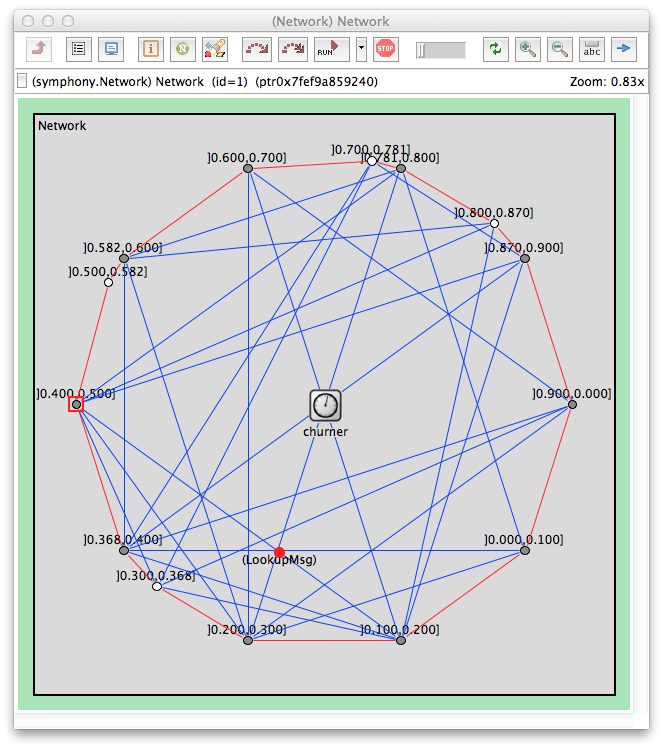
\includegraphics[scale=0.32]{imgs/screenshot.png}
\caption{Una screenshot della simulazione. Possiamo notare i long link colorati di blu ed i short link colorati di rosso. I nodi più scuri sono i peer statici, mentre quelli più chiari sono quelli dinamici. Ogni peer ha poi una label che indica il range di valori che vengono amministrati da tale nodo.}
\end{center}
\end{figure}

\subsection{Il simulatore di Symphony}

La simulazione è costituita da una rete, contenente una serie di peer configurabili nel numero, collegati tra loro attraverso dei canali di comunicazione. Inoltre il simulatore comprende un'entità speciale, diversa dal peer, chiamata \emph{Churner}, che gestisce l'entrata e l'uscita dei peer secondo due parametri configurabili relativi rispettivamente alla \emph{frequenza di entrata} (\texttt{join\_freq}), alla \emph{frequenza di uscita} dei peer (\texttt{leave\_freq}) e al numero di peer cui viene chiesto di entrare contemporaneamente ad ogni ciclo di churn (\texttt{concurrent\_joins\_per\_freq}). Questa è la componente che permette di simulare il churn e quindi di misurare conseguentemente la stabilità del protocollo.

Il peer rappresenta un generico nodo della rete. Esso mantiene alcune informazioni fondamentali:
\begin{itemize}
	\item ~Un id $id_i \in [0,1)$, che identifica univocamente il peer $p_i$ all'interno della rete di overlay Symphony.
	\item ~Un canale di comunicazione verso il nodo precedente, ed un altro verso il successivo. Questi costituiscono gli \textit{short link} di Symphony.
	\item ~Un array di canali di comunicazione verso peer arbitrari della rete. Questi costituiscono i \textit{long link} di Symphony.
\end{itemize}

Inoltre ogni peer può contare su una serie di parametri identici per ogni peer, che delineano in modo parametrico il loro comportamento finale:
\begin{itemize}
	\item ~Il parametro \textit{k}, che costituisce il numero di long link che il peer deve provare a instaurare.
	\item ~Un parametro per stabilire il numero di tentativi che il peer è disposto a fare per costruire i long link. Ciò viene accuratamente descritto nell'articolo originale di Symphony.
	\item ~Un parametro che indica se il peer utilizza il protocollo di \emph{re-linking} o meno.
\end{itemize}

Inoltre, ai fini della simulazione del churn, i peer sono suddivisi in due classi distinte: i peer \emph{statici} e i peer \emph{dinamici}. Descriviamo nel seguito le caratteristiche delle due classi di peer.

\subsubsection*{Peer statici}
Un peer statico è un peer che entra nella rete all'inizio della simulazione e non esce più dalla rete. Esso quindi non fa parte dei peer gestiti dal Churner. Ogni peer statico $p_i$ ha un $id_i \in [0,1)$ deterministico uniformemente distribuito nell'anello: se rappresentiamo i peer statici come $\{p_1, \linebreak[1] p_2, \linebreak[1] ..., \linebreak[1] p_n\}$, abbiamo che $id_i = i / n$.

Gli short link dei peer statici vengono definiti direttamente nel file NED. I long link, invece, non possono essere definiti nel file NED a causa del potere espressivo troppo debole del linguaggio NED stesso. Sarebbe infatti possibile costruire soltanto un'approssimazione dei long link, la quale non garantirebbe l'assenza di conflitti (ad esempio, un long link che collega due nodi già connessi), né tantomeno si garantirebbe la conformità al protocollo Symphony (ad esempio, non si potrebbe implementare il massimo numero di tentativi per la creazione dei long link, che permette di risolvere situazioni di rete satura). Pertanto, i long link vengono creati dagli stessi peer statici all'inizio della simulazione, senza l'utilizzo di messaggi. In questo modo, è necessario attendere un breve periodo, chiamato \textit{periodo di warmup}, prima di poter registrare i dati della simulazioni. In particolare, il Churner deve attendere tale periodo prima di iniziare la fase di churn.

\subsubsection*{Peer dinamici}
I peer dinamici vengono inseriti nella rete solo quando deciso dal Churner. All'inizio, quindi, essi si trovano all'esterno della rete di overlay, e non stabiliscono né short link né long link.

Un peer dinamico rimane quindi in disparte fino a quando il Churner, attraverso un messaggio, non gli chiede di entrare a far parte della rete. A quel punto, come stabilito da Symphony, questi calcola il suo id $x$ e individua l'attuale manager di $x$ attraverso un lookup, contattando un nodo della rete noto a priori (un nodo casuale tra quelli statici, scelta che garantisce uniformità nel carico in questa prima fase).

Un peer dinamico, dopo essere entrato all'interno della rete di overlay, rimane al suo interno fintantoché il Churner non gli chiede di uscire. A quel punto il peer non deve far altro che eliminare tutti i collegamenti, ripristinando la topologia, e ritornare nella sua fase iniziale, attendendo nuovamente di poter rientrare. 

Quando il peer dinamico si trova fuori dalla rete, può ricevere comunque dei messaggi (ad esempio, quelli che gli sono stati mandati poco prima la sua uscita, ancora in transito al momento dell'uscita). Tali messaggi verranno scartati dal peer e rimandati al mittente, in modo da simulare fedelmente ciò che accadrebbe nella realtà (si pensi ai tempi di attesa nel caso in cui provassimo a contattare un nodo esistente che non vuole accettare una richiesta di connessione). In tal modo, il mittente potrà re-inviare il messaggio al peer più appropriato (si pensi ad esempio al lookup).

\subsubsection*{Il Churner}
Il Churner è l'entità esterna alla rete di overlay che gestisce il churn. Le sue funzionalità base sono: (1) comunicare ogni \texttt{join\_freq} secondi a \texttt{concurrent\_joins\_per\_freq} peer dinamici scelti casualmente tra quelli all'esterno della rete di entrare e (2) comunicare ogni \texttt{leave\_freq} secondi ad un peer dinamico scelto casualmente tra quelli già entrati nella rete di uscire. Il Churner quindi partiziona l'insieme dei peer dinamici in quattro sottoinsiemi: i peer esterni alla rete e che non stanno entrando, i peer esterni cui è stato chiesto di entrare e che stanno completando le operazioni di join, i peer entrati nella rete e che non stanno per uscire, e infine i peer dentro la rete cui è stato chiesto di uscire e che stanno completando le operazioni di uscita.

La scelta di gestire il churn attraverso questa entità esterna è motivata dal fatto che lasciare che siano i peer stessi a gestire le loro entrate e uscite richiederebbe l'implementazione di una complessa coordinazione tra di loro. Il Churner offre un controllo del churn più flessibile, semplice e potente.


\subsection{Il livello di astrazione e i messaggi}

%simulazione della sola rete di overlay
Una prima osservazione riguarda la topologia della rete simulata. Come viene solitamente fatto nelle simulazioni riguardanti reti di overlay peer-to-peer, la simulazione astrae da dettagli relativi alla reale topologia fisica dei nodi, ovvero la loro effettiva distribuzione nel territorio. Inoltre, vengono ignorati tutti i dettagli relativi ai protocolli di comunicazione di più basso livello (ad esempio TCP/IP). La simulazione presenta solamente un delay dei canali di comunicazione di 100ms e un bandwith di 10Mbps, che stimiamo essere una buona approssimazione di un tipico canale di comunicazione su Internet.

%La simulazione, come abbiamo precedentemente visto, è composta dai vari peer, collegati tra di loro mediante gli short link ed i long link. Una prima osservazione sul livello di astrazione è pertanto quella che riguarda la topologia della rete che collega tali peer. Nella realtà, ogni peer fa parte della rete reale di Internet, che è differente dalla rete di overlay logica creata da Symphony. Nella nostra simulazione, viene rappresentata solamente quest'ultima, dove ogni link (sia short che long) ha un delay di 100ms ed un bandwith di 10Mbps, che stimiamo essere una buona approssimazione di un usuale canale di comunicazione logico, che colleghi due peer presenti sulla rete di Internet.

%come abbiamo risolto gli accessi a sezioni critiche
In una reale implementazione del protocollo, i peer che entrano ed escono dalla rete hanno bisogno di meccanismi di accesso in sezione critica distribuiti per non creare delle incoerenze che potrebbero intaccare negativamente la struttura della rete di overlay. Tali meccanismi sono a volte complessi da implementare e non sono oggetto del nostro studio. È stato pertanto sfruttato il fatto che il simulatore genera eventi discreti mai gestiti in concorrenza tra loro (il simulatore non è parallelo). Tutte le manipolazioni della topologia vengono fatte dal peer interessato, in un solo metodo, compiendo pertanto azioni atomiche. Per esempio, si consideri il caso di un peer $p$ che vuole entrare nella rete con un id $x$. Nella nostra simulazione, è l'attuale manager di $x$ colui il quale modifica gli short link per far entrare $p$ all'interno della rete, diversamente da come dovrebbe avvenire in una reale implementazione del protocollo.

%conoscenza del vicinato
Si assume inoltre che ogni peer abbia conoscenza dei peer che compongono il proprio vicinato (due nodi per gli short link e al più sei per i long link). Questa è un'assunzione realistica, comunemente utilizzata nei reali sistemi peer-to-peer. In questo modo ogni peer conosce con esattezza il sotto-intervallo da esso gestito, nonché quale dei propri vicini gestisce l'id più vicino ad una certa $x$, nel momento in cui è necessario un foward per il protocollo di routing. In una reale implementazione queste due considerazioni continuerebbero a valere, rendendo questi aspetti fedelmente emulati.
%Ogni peer conosce pertanto l'id di ogni suo vicino, recuperato al momento della creazione del link che li ha connessi. Lo stesso non si può dire per gli id gestiti da un peer vicino, poiché in questo caso tale informazione cambia continuamente. 

%che id gestisco? qual'è il peer vicino migliore per forwardare un messaggio?
%Ciò è necessario per chiarire due due cose molto importanti. La prima è sapere quali sono gli id gestiti dal proprio peer: tale informazione viene ottenuta senza l'invio di nessun messaggio, considerando il proprio id e quello del peer precedente. La seconda è sapere a chi dobbiamo fare il forward di un messaggio di lookup che richiede di cercare il manager dell'id $x$. Anche in questo caso, senza mandare messaggi, possiamo semplicemente controllare gli id di ogni peer vicino, e fare il forward al peer con l'id più vicino ad $x$, rispettando le specifiche del Routing Protocol descritto da Symphony. In una reale implementazione queste due considerazioni continuerebbero a valere, rendendo questi aspetti fedelmente emulati.

\subsubsection*{Messaggi}

Ogni peer può mandare e ricevere diversi messaggi:
\begin{itemize}
	\item ~\texttt{LookupMsg}: è il messaggio di lookup. Tale messaggio può essere utilizzato per tre motivi diversi: per cercare il manager di un id quando viene fatto un join, per cercare il manager di un id per poter creare un long link, oppure per un lookup generico che simula la ricerca di un file all'interno della rete.
	\item ~\texttt{LookupResponseMsg}: è la risposta ad un lookup, che trasporta al suo interno l'identificatore del manager. In questo modo il peer che ha fatto la richiesta può compiere un'azione opportuna.
	\item ~\texttt{NEstimationMsg}: è il messaggio che viene spedito per aggiornare la stima del numero di peer presenti all'interno della rete, come previsto dal protocollo di Symphony.
\end{itemize}

%id nei messaggi di lookup, coda dei messaggi di uscita
Ogni richiesta di lookup emessa da un determinato peer viene identificata con un id crescente. Anche nel caso in cui un peer uscisse e rientrasse nella rete, tale id è garantito essere distinto.
Ogni peer mantiene inoltre la coda dei lookup richiesti, associando ad ognuno di essi la corrispettiva procedura di callback da eseguire al termine del lookup.
%Ogni risposta ad un lookup (cioè, un \texttt{LookupResponseMsg}) mantiene al suo interno questi id, permettendo al peer, grazie alla coda, di identificare e continuare a svolgere la procedura che aveva richiesto il lookup (il messaggio viene ignorato se non si dovesse trovare nella coda una corrispondenza).
Tale coda viene svuotata al momento dell'uscita del peer dalla rete, permettendo di ignorare le risposte a lookup inviati in una precedente reincarnazione del peer.

%join
%Per utilizzare i messaggi di lookup in modo da effettuare un join, il peer segna in maniera opportuna un campo all'interno del messaggio stesso, in modo da distinguerlo. Così facendo, il manager dell'id, invece di rispondere solamente a tale lookup, può manipolare la topologia della rete di overlay, in modo da far entrare il peer al suo interno. Le operazioni di join non possono infatti essere fatte dal peer stesso, poiché, durante il tempo trascorso per la ricezione della risposta del lookup, il manager può non gestire più l'id che gli era stato richiesto, generando conflitti che perturberebbero la topologia della rete di overlay. Il join, compiendo un'azione atomica per manipolare la topologia, utilizza pertanto un numero di messaggi che nella realtà sarebbe più alto. 

Nel caso in cui un lookup sia stato chiesto per effettuare un join con id $x$ (ovvero, il primo lookup chiesto da ogni peer), il messaggio di lookup contiene un campo opportuno che segnala al manager di $x$ di effettuare le operazioni di creazione degli short link. Ciò ha l'unico scopo di evitare, come discusso in precedenza, l'implementazione di una sezione critica distribuita non oggetto del presente studio.

%leave
Le operazioni relative al leave vengono fatte dal peer in maniera atomica, anche qui sfruttando il concetto discusso precedentemente, in modo da evitare gestione complessa della concorrenza. Come nel caso del join, il numero di messaggi inviati è minore di quello che sarebbe necessario in una reale implementazione del protocollo.









\section{Risultati sperimentali} \label{risultati}
Riportiamo in questa Sezione i risultati sperimentali sulla stabilità del protocollo Symphony, derivanti dalle simulazioni realizzate per mezzo del nostro simulatore.

\subsection{Validazione del simulatore}

\begin{figure}	
\minipage{0.50\textwidth}
\centering
	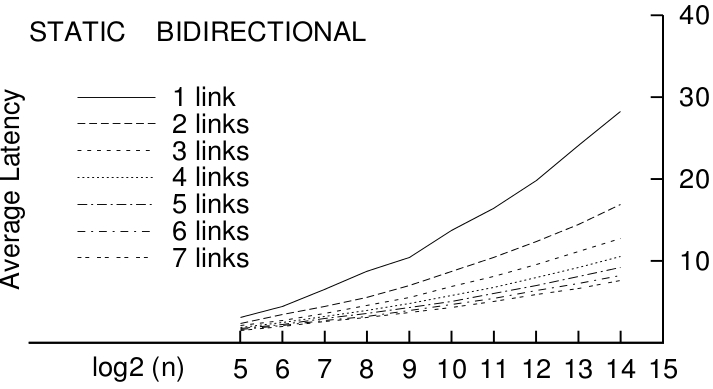
\includegraphics[scale=.31]{imgs/join-reale.jpg}
\endminipage\hfill
\minipage{0.50\textwidth}
\centering
	\includegraphics[scale=.31, angle=-90]{imgs/join_cost.eps}
\endminipage\hfill
\caption{Validazione del simulatore: a sinistra le latenze medie registrate nel paper originale, a destra quelle registrate utilizzando il nostro simulatore. In entrambi i casi, i tempi di latenza sono polilogaritmici.}
\label{img:join-cost}
\end{figure}

Il primo esperimento che riportiamo è atto a supportare la validazione del simulatore realizzato. La validazione effettuata riguarda il protocollo di routing. Nel paper originale, il numero dei peer nella rete viene fatto variare da $2^5$ a $2^{14}$ e vengono misurati gli hop medi per lookup, facendo anche variare $k$ (il numero massimo di long link uscenti). Nel nostro caso, invece, $k$ è stato tenuto fisso a $3$, un valore che gli autori stimano essere ottimo per l'ottenimento di basse latenze. Il nostro simulatore inoltre utilizza solamente il routing bidirezionale, come precedentemente accennato.

In Figura~\ref{img:join-cost} mettiamo a paragone i risultati delle simulazioni del paper originale (a sinistra) con quelli del nostro simulatore (a destra). Ogni punto della Figura relativa al nostro simulatore è il risultato della media di 10 run di simulazione, ognuno dei quali ha registrato il numero di hop di 100 lookup. Dalla Figura è evidente come l'andamento della curva relativa alla latenza media dei lookup sia identico nei due simulatori (nonostante una differenza nelle costanti dovuta alla diversa implementazione), ovvero polilogaritmico nel numero dei peer presenti nella rete. Questo risultato è utile per validare il nostro protocollo di routing simulato per mezzo di Omnet++, come precedentemente descritto. La Figura mostra anche come gli intervalli di confidenza, misurati al 95\%, con distribuzione t-student, siano abbastanza piccoli da reputare la media un valore attendibile, il che contribuisce a validare i risultati.

\subsection{Stabilità senza re-linking}
% Al variare di frequenza
% Al variare del numero di peer che entrano nello stesso tempo: discutere della velocità di crescita di N rispetto alla velocità di decrescita di H
Il primo esperimento atto a valutare la stabilità di Symphony riguarda l'analisi degli effetti relativi all'aumentare della frequenza del numero dei peer che effettuano join nella rete.
Il Churner, in questo esperimento, chiede ad un peer di entrare ogni \texttt{join\_freq} secondi, e ad un altro di uscire ogni \texttt{leave\_freq} secondi. Nel momento in cui ad un peer viene chiesto di entrare, esso comincia la prima procedura di lookup del manager relativo al suo nuovo id. Solo dopo averlo trovato, il peer si unisce alla rete, inizialmente utilizzando soltanto due short link, in modo da chiudere l'anello. In quel momento, comincia la sua procedura di creazione dei long link, la quale terminerà solo dopo averne creato un numero sufficiente, secondo le specifiche di Symphony.

Al fine di misurare la stabilità del protocollo Symphony secondo le definizioni di stabilità presentate in Sezione~\ref{stabilita}, sono stati svolti due test. Nel primo test viene calcolato il valore di $stability(H,N)$ al variare della frequenza del churn. Nel secondo test viene calcolato lo stesso valore al variare del numero di peer che stanno entrando contemporaneamente nella rete. I due test, sebbene possano sembrare simili, evidenziano caratteristiche diverse relativamente alla nostra definizione di stabilità, le quali saranno più chiare nel resto della trattazione.


\subsubsection{Stabilità al variare della frequenza dei join}

Nei primi test che riportiamo in questa Sezione, la rete viene stressata controllando la frequenza a cui viene chiesto ai peer di entrare e uscire dalla rete.
È proprio durante questa fase che la rete può mostrare potenziali segni di instabilità. Se il peer appena entrato è l'unico con soli short link, l'effetto della mancanza dei suoi long link non sarà particolarmente evidente nella totalità delle misurazioni.
Di contro, se vi è un numero considerevole di peer in fase di creazione di long link, il numero degli hop per lookup in media può aumentare considerevolmente. Nel caso pessimo, come discusso in precedenza, tale numero è $O(n)$, quando il routing del lookup incontra soltanto peer senza long link instaurati.

\begin{figure}	
\minipage{0.33\textwidth}
\centering
	\includegraphics[scale=.22, angle=-90]{imgs/norelink-freq-hops.eps}
\endminipage\hfill
\minipage{0.33\textwidth}
\centering
	\includegraphics[scale=.22, angle=-90]{imgs/norelink-freq-time.eps}
\endminipage\hfill
\minipage{0.33\textwidth}
\centering
	\includegraphics[scale=.22, angle=-90]{imgs/norelink-freq-percLongLinks.eps}
\endminipage\hfill
\caption{Latenza media (a), tempi medi (b) e percentuale dei long link creati (c) al variare della frequenza del join, senza re-linking.}
\label{img:stabilita}
\end{figure}

In Figura~\ref{img:stabilita} mostriamo i risultati del primo test, in cui variamo la frequenza dei join in modo crescente.
In tutte le simulazioni sono stati utilizzati 32 peer statici (ovvero, entrati prima dell'inizio delle registrazioni e mai usciti dalla rete) e 8 peer dinamici. Gli 8 peer dinamici sono stati fatti entrare e uscire 2048 volte. In questo modo è stato possibile aggregare molti valori registrati dallo stesso peer. Una volta che uno di questi peer è entrato e ha completato tutta la sua fase di creazione dei long link, il Churner gli ha chiesto di uscire dopo 0.1ms. La frequenza di entrata, invece, è stata fatta variare da 1 peer ogni $10^6$ millisecondi ad 1 peer ogni $10^{-8}$ millisecondi. Ogni punto rappresentato nella curva in Figura è il risultato della media di 10 run di simulazione.

Nel primo test, riportato in Figura~\ref{img:stabilita}(a), mostriamo la latenza media dei lookup (ovvero, il numero medio degli hop). Con join poco frequenti (fino a un join al secondo) il numero di hop medi è estremamente basso, ovvero circa 1 e mezzo. Nel momento in cui viene chiesto un join ogni 100ms ecco che il numero di hop inizia a crescere. Ciò è motivato dal fatto che 100ms non sono sufficienti ai peer per poter instaurare tutti i loro long link, col risultato che la rete in quel momento risulta non completa. Una rete non completa non è in grado quindi di garantire il numero di hop poli-logaritmico, come discusso in precedenza. Il grafico in Figura~\ref{img:stabilita}(b) mostra i tempi medi di lookup, calcolati in secondi. Come ci aspettavamo, i tempi hanno un andamento pressoché identico a quello della latenza media, in quanto i pacchetti di lookup sono lunghi solamente una decina di byte, troppo pochi per saturare i molteplici canali esistenti nella rete. Inoltre, simulando solamente la rete di overlay, non vengono simulate congestioni o ritardi impredicibili della rete fisica.

Al fine di validare la nostra ipotesi, abbiamo effettuato un ulteriore esperimento in cui abbiamo calcolato la percentuale di long link già creati dai peer presenti nella rete. In Figura~\ref{img:stabilita}(c) è evidente come in corrispondenza della frequenza di join che causa un aumento netto del numero degli hop vi sia un calo netto nella percentuale di long link presenti nella rete. Addirittura, tale percentuale scende sotto il 20\%. È evidente come una rete con meno del 20\% dei long link non sia in grado di garantire una latenza media bassa. Questo è il primo segno di instabilità del protocollo Symphony.

\begin{figure}	
\centering
	\includegraphics[scale=.35, angle=-90]{imgs/norelink-freq-stability.eps}
\caption{Stabilità al variare della frequenza del join, senza re-linking.}
\label{img:stabilita2}
\end{figure}

Infine, in Figura~\ref{img:stabilita2} mostriamo i valori della stabilità calcolati al variare della frequenza di join. Ogni punto della curva di stabilità è un valore $stability(H_i,N_i)$, corrispondente all'$i$-esima frequenza di join, tale che $H_i = \{ h_1, h_2, \dots, h_{10} \}$ e $N_i = \{ n_1, n_2, \dots, n_{10} \}$ per 10 run di simulazione nei quali $h_j$ e $n_j$ sono rispettivamente il numero di hop medi e il numero di peer medi misurati al $j$-esimo run.
Dalla Figura è evidente come la stabilità diminuisca nettamente in corrispondenza dell'aumento della latenza, ovvero dal momento in cui viene fatto entrare un peer ogni 100ms.

I grafici qui presentati mostrano come la stabilità del protocollo sia effettivamente minata dalla frequenza del fenomeno di churn. Ciononostante, essi non mettono in relazione la stabilità con il numero di nodi presenti nella rete, come invece evidenziato nella stabilità teorica discussa nelle Sezioni precedenti. In particolare, essi non mostrano l'effetto di più peer che tentano di entrare nella rete tutti nello stesso momento. Questo breve ragionamento ha motivato la necessità di sviluppare ulteriori esperimenti, presentati qui di seguito.
%La stabilità misurata in questo modo, purtroppo, non è tale da permetterci di trarre particolari conclusioni. Infatti, all'aumentare della frequenza dei join, anche il numero di peer nella rete aumenta. Essendo la stabilità proporzionale al numero di peer nella rete, essa aumenta in funzione del numero di nodi.



\subsubsection{Analisi rispetto alla stabilità teorica}
Al fine di valutare in maniera più esaustiva la stabilità del protocollo, è stato effettuato un diverso tipo di test, in cui non è la frequenza dei join a variare, ma il numero dei peer che tentano di entrare nella rete nello stesso istante. Ciò permette di mettere a paragone la stabilità del protocollo rispetto alla stabilità teorica, ed evidenziare ulteriori indizi di instabilità.

Come detto in Sezione~\ref{stab-teorica}, la stabilità del protocollo in una rete di $n$ nodi completa (ovvero in cui tutti i long link sono stati instaurati) è garantita essere superiore o uguale a $1 - \frac{log^2n}{k \cdot n}$. Ciononostante, la stabilità misurata su una rete non ancora completa può essere inferiore a questo lower bound. È quindi importante valutare se il protocollo è in grado di mantenere la propria stabilità vicina al proprio lower bound teorico anche in situazioni di stress causate da un numero elevato di peer che tentano di entrare nella rete tutti nello stesso momento.

\begin{figure}
\includegraphics[scale=.32, angle=-90]{imgs/norelink-conc-stability2-hops.eps}
\includegraphics[scale=.32, angle=-90]{imgs/norelink-conc-stability2-stab.eps}
\caption{Latenza media e stabilità per numero di peer crescente, senza re-linking.}
\label{img:norelink-conc}
\end{figure}

La simulazione mostrata in Figura~\ref{img:norelink-conc} è stata realizzata facendo variare il numero di peer che chiedono di fare join nella rete nello stesso istante e che tentano di instaurare $k=2$ long link. All'inizio di ogni run la rete contiene solo 5 peer statici. Ad ogni run viene chiesto a $2^{i}$ peer di entrare nello stesso momento, per $i$ che varia tra $0$ e $12$. Nessun peer esce, quindi la rete non fa altro che crescere. Il numero dei peer registrato (e riportato nell'asse $x$) comprende tutti i peer già entrati così come i peer che stanno per entrare sia con gli short link che con i long link. Ogni punto della curva è stato calcolato sulla base dei risultati di 10 run.

L'immagine a sinistra mostra il numero di hop medi per i lookup. I risultati in questo caso sono molto simili a quelli della Figura~\ref{img:join-cost}, con l'unica differenza che gli intervalli di confidenza sono talvolta leggermente più larghi e variabili, dati dall'intensa attività del churn non attivo nel test precedente. Questa Figura mostra anche come sia poco informativo guardare soltanto al numero di hop in relazione al numero dei nodi della rete al fine di valutare la stabilità del protocollo. Infatti, guardando il grafico in questione non è possibile valutare la stabilità del protocollo di Symphony, il che giustifica ulteriormente la nostra scelta di definire la stabilità con una misura che aggrega sia il numero degli hop che il numero dei nodi nella rete.

Il grafico di destra in Figura~\ref{img:norelink-conc} è invece ricco di spunti informativi sulla stabilità del protocollo. Il grafico mostra la stabilità teorica insieme alle stabilità misurate attraverso la simulazione: stabilità medie, minime e massime. Per la stabilità media sono stati anche riportati gli intervalli di confidenza calcolati al 95\% con distribuzione t-student. Sono molteplici le considerazioni che si possono trarre dal grafico in questione.

Innanzitutto, è evidente come la stabilità media sia conforme in generale alla stabilità teorica, il che è un ulteriore prova della validità del simulatore e dei test realizzati con esso. Come previsto dalla teoria, la stabilità inizialmente diminuisce, toccando il suo minimo quando circa 8 nodi sono presenti nella rete. Dopodiché, all'aumentare dei nodi, essa comincia ad aumentare logaritmicamente, grazie al fatto che all'aumentare dei nodi connessi aumenta il contributo generale al raggiungimento delle condizioni ottimali per i lookup logaritmici.

I valori di stabilità massima sono più che soddisfacenti. Ciononostante, i valori minimi illustrano che il protocollo comincia a mostrare i primi segni di cedimento più seri già con 32 nodi. I minimi rimangono sempre sotto la soglia del lower bound teorico da quel punto in poi. I valori medi, invece, evidenziano un calo di stabilità a partire da 512 nodi. Ad ogni modo, i valori misurati si tengono sempre di poco al di sotto del lower bound teorico, dimostrando come la perdita di stabilità sia molto controllata.

Infine, è bene notare come le differenze tra minimi e massimi, così come l'ampiezza degli intervalli di confidenza relativi ai valori medi siano maggiori con reti piccole (fino a circa 64 nodi), mentre la stabilità cominci a convergere mano a mano che la rete cresce (da 128 nodi in poi). Ciò significa che nonostante il protocollo risenta dell'elevato numero di peer che entrano tutti contemporaneamente, più ve ne sono più le probabilità che essi comincino presto a contribuire alla stabilità del protocollo aumentano.





\subsection{Stabilità con re-linking}
% Come prima: mostra che non cambia molto perché relinking non scatta
% Mostra che cambiando alcuni parametri si fa scattare il relinking e le cose peggiorano molto
Come discusso nel paper originale di Symphony, il protocollo di re-linking prevede la distruzione e la creazione di nuovi long link ogniqualvolta la stima corrente del numero dei nodi della rete cambi di molto rispetto alla stima relativa al precedente re-linking. Ciò ha il beneficio di re-instaurare long link corretti, che meglio si adattano alla nuova rete, una volta che questa abbia subito ingenti cambiamenti nel numero di peer. Inoltre, il re-linking gestito per mezzo di soglie ha il vantaggio di ridurre notevolmente il numero di peer che fanno re-linking contemporaneamente. Gli esperimenti effettuati dagli autori di Symphony mostrano come il re-linking sia effettivamente poco costoso (poiché attivato di rado e da pochi peer alla volta), ma che i benefici apportati per quanto riguarda la latenza media dei lookup sia solo marginale.

\begin{figure}
\includegraphics[scale=.32, angle=-90]{imgs/relink-conc-stability2-hops.eps}
\includegraphics[scale=.32, angle=-90]{imgs/relink-conc-stability2-stab.eps}
\caption{Latenza media e stabilità per numero di peer crescente, con re-linking attivo.}
\label{img:relink-conc}
\end{figure}

L'effetto del re-linking è invece evidente nelle misurazioni della stabilità del protocollo. Dato che il re-linking distrugge i long link per crearne di nuovi, si potrebbe supporre che la sua attivazione giochi a sfavore della stabilità del protocollo. In realtà invece, è l'esatto contrario, come dimostrano gli esperimenti delle simulazioni mostrate in Figura~\ref{img:relink-conc}. L'esperimento è analogo al precedente test in cui la stabilità misurata viene messa a paragone con quella teorica, con l'unica differenza che stavolta il protocollo di re-linking è attivo.

La Figura conferma i risultati del paper originale circa il guadagno molto marginale dato dal re-linking in termini della latenza media (figura a sinistra), che conferma ulteriormente la necessità di una definizione di stabilità dipendente dal numero dei peer nella rete, come quella da noi proposta. L'esperimento mostra come il re-linking dia invece benefici evidenti sulla stabilità (figura a destra), già a partire da reti con pochissimi nodi. L'effetto del re-linking è quello di far sì che i lookup continuino ad essere poli-logaritmici anche in seguito alla crescita della rete. Per questo motivo, i valori di stabilità minimi e medi sono generalmente migliori quando il re-linking è attivo. In particolare, la stabilità media comincia a peggiorare rispetto al lower bound teorico solo quando vi sono 1024 nodi contemporaneamente intenti a fare join, a differenza dei 512 nodi sufficienti nel caso di protocollo senza re-linking.

È inoltre interessante osservare come la curva con re-linking sia più omogenea rispetto a quella senza re-linking. Ciò avviene perché il re-linking garantisce una maggior vicinanza tra i valori misurati e i bound teorici del protocollo e, nella fattispecie, garantisce un comportamento meno variabile della stabilità, più simile a quello della curva data dalla stabilità teorica di Symphony.

Infine, il test dimostra nuovamente che il protocollo Symphony comincia a perdere un po' di stabilità non appena la rete cresce oltre una certa soglia (1024 nodi nella Figura). Ciò rafforza i risultati precedenti, in quanto il fatto che il re-linking aggiusti le latenze medie non è sufficiente a garantirne una stabilità al di sopra della soglia minima teorica. Infatti, tale perdita di stabilità non viene evitata nemmeno dal protocollo di re-linking.



\subsection{Gli $\epsilon^*$ di Symphony}
Riportiamo infine i valori di $\epsilon^*$ di Symphony calcolati sulla base delle precedenti simulazioni. Ricordiamo che la stabilità di un protocollo di DHT è stata definita in base ad un parametro $\epsilon$, requisito di stabilità dell'applicazione. Il valore $\epsilon^*$ è il minimo valore di $\epsilon$ per cui il protocollo è stabile. Più basso è il valore di $\epsilon^*$ più il protocollo è da considerarsi stabile.

Il valore di $\epsilon^*$ calcolato sulla base della simulazione riportata in Figura~\ref{img:stabilita2} è $0.313$.
Un effetto simile sul valore di $\epsilon^*$ si ha al variare del numero di peer che entrano nella rete contemporaneamente. Il valore calcolato sulla base degli esperimenti in Figura~\ref{img:norelink-conc} (senza re-linking) è $0.119$. L'esperimento ha infatti messo in luce, anche in questo caso, una leggera instabilità del protocollo. Il valore calcolato invece sullo stesso esperimento in cui il protocollo di re-linking è stato attivato (ovvero l'esperimento della Figura~\ref{img:relink-conc}) mostra un $\epsilon^*$ più basso, pari a $0.089$. Ciò è in linea con quanto discusso in precedenza, ovvero col fatto che il re-linking aumenti leggermente la stabilità del protocollo.



\section{Conclusioni} \label{conclusioni}

Nella presente relazione abbiamo analizzato approfonditamente la stabilità del protocollo di DHT Symphony in relazione al fenomeno di churn, un aspetto che è stato analizzato solo in maniera marginale dagli autori del protocollo. 

Dopo aver brevemente riassunto gli aspetti chiave di Symphony che abbiamo ritenuto fondamentali per condurre uno studio della stabilità del protocollo,
abbiamo introdotto una nuova nozione di stabilità, adatta non solo al protocollo in questione, ma ad un qualsiasi protocollo di DHT. Tale definizione, può essere infatti utilizzata per valutare la stabilità di altri protocolli, nonché per mettere a paragone la stabilità di protocolli differenti. Più precisamente, sono state fornite tre definizioni correlate: la prima riguarda la stabilità di un singolo lookup, la seconda riguarda la stabilità di un insieme di misurazioni, mentre l'ultima riguarda la stabilità di un protocollo DHT sulla base di una serie di misurazioni atte a stressare il sistema.

Al fine di fornire un quadro completo sulle simulazioni effettuate, abbiamo discusso gli strumenti utilizzati e il livello di astrazione che ha guidato l'implementazione del simulatore. Ciò ha permesso di sottolineare quali fossero le parti simulate fedelmente e quali quelle semplificate poiché ritenute poco interessanti per il nostro studio.

Infine, abbiamo mostrato e discusso i risultati di una serie di test. Il primo test effettuato riguarda la validazione del sistema, in particolare del protocollo di routing simulato. Il secondo test, effettuato senza re-linking, mostra come la latenza cresca all'aumentare della frequenza di churn e che al relativo tipping point corrisponda una diminuzione netta della stabilità motivata dall'assenza in gran parte della rete dei long link necessari a garantire i lookup logaritmici.

Un diverso tipo di test, dove a variare non è la frequenza di join ma il numero di peer che entrano contemporaneamente nella rete, ha invece permesso di mostrare come la stabilità teorica si rapporti a quella sperimentale misurata per mezzo del simulatore. Tale test è anche un'ulteriore conferma della validità del simulatore realizzato, in quanto l'andamento della stabilità misurato sperimentalmente è consono all'andamento teorico valutato analiticamente. Esso è inoltre un importante spunto di riflessione atto a sottolineare come la latenza media non sia un parametro da solo sufficiente ad analizzare la stabilità di un protocollo DHT.

L'ultimo test è stato ri-effettuato utilizzando il protocollo di re-linking. A differenza di come si era pronosticato, tale protocollo invece di causare un degrado della stabilità, ne causa un netto miglioramento, poiché permette al sistema di garantire long link di ottima qualità.

Per finire abbiamo calcolato il valore di $\epsilon^*$ di Symphony, in modo tale da permettere una comparazione della stabilità dello stesso con altri protocolli DHT, attraverso le definizioni di stabilità introdotte nella presente relazione. Sarebbe pertanto interessante poter continuare in tal senso il lavoro di comparazione qui soltanto accennato.

TODO: mega conclusioni finali? è buono sympnohy?












% Appendix
%\appendix
%\section*{APPENDIX}
%\setcounter{section}{1}



% Bibliography
\bibliographystyle{ACM-Reference-Format-Journals}
\bibliography{bibliografia}

% History dates
%\received{February 2009}{July 2009}{October 2009}




%\elecappendix


%\section{Analysis of Invalid Trials}
%\label{invalid}

%\subsection{Results}




\end{document}
% End of v2-acmlarge-sample.tex (March 2012) - Gerry Murray, ACM
